\documentclass[a4paper,11pt,oneside]{article}

\usepackage{amsmath,amssymb,epsfig}
\usepackage[T1]{fontenc}
\usepackage{ae,aecompl}
\usepackage{url}
\usepackage{subfigure}
\addtolength{\voffset}{-.5cm}
\addtolength{\hoffset}{-.5cm}
\setlength{\parindent}{0in}
\addtolength{\textwidth}{.5cm}
\addtolength{\textheight}{.51cm}
\addtolength{\parskip}{.5cm}

% Example definitions.
% --------------------
\def\e{{e^{j\omega}}}
\def\W{{W_M}}
\def\sumk{{\sum_{k=-\infty}^{\infty}}}
\def\x{{\mathbf x}}
\def\X{{\mathbf X}}
\def\Y{{\mathbf Y}}
\def\u{{\mathbf u}}
\def\U{{\mathbf U}}
\def\x{{\mathbf x}}
\def\s{{\mathbf s}}
\def\A{{\mathbf A}}
\def\y{{\mathbf y}}
\def\w{{\mathbf w}}
\def\B{{\mathbf B}}
\def\a{{\mathbf a}}
\def\D{{\mathbf D}}
\def\P{{\mathbf P}}
\def\n{{\mathbf n}}
\def\V{{\mathbf V}}
\def\R{{\mathbf R}}
\def\I{{\mathbf I}}
\def\M{{\mathbf M}}
\def\sech{{\mathrm{sech}}}
\def\L{{\cal L}}
\def\Cum{{\rm{Cum}}}
\def\var{{\rm{var}}}
\def\T{{\mathbf T}}
\def\C{{\mathbf C}}
\def\tf{{\emph{t-f}}}


% Title.
% ------
\title{SGN-1107 Introductory Signal Processing\\
Sample exam}
%
% Author and date.
% ---------------
\author{Germ\'an G\'omez-Herrero, \url{http://germangh.com}}
\date{\today}



\begin{document}
\maketitle


\textbf{NOTE:} This solutions are explained in great detail to be sure that you understand every step taken. When you do your exam you SHOULD NOT go into so much detail. It is enough to show the major intermidiate steps.

\vspace{1cm}

\textbf{QUESTION 1 (5 point):} Consider the following interconnection of linear shift-invariant systems:

\begin{figure}[h!]
\centering
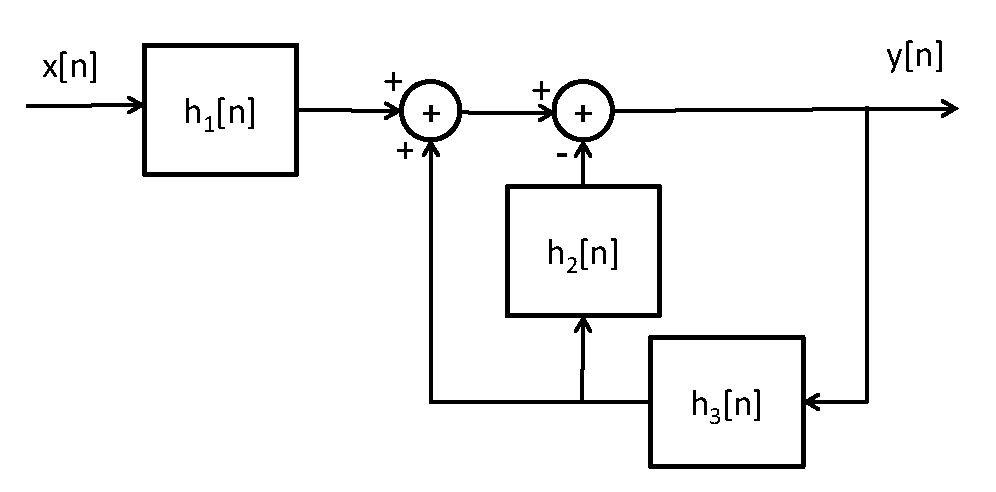
\includegraphics[width=.8\textwidth]{fig1.eps}
\end{figure}

\begin{itemize}
\item[(a)] (3 points) Express the overall frequency response of the overall system $H(e^{j\omega})$ in terms of the frequency responses of the subsystems $H_1(e^{j\omega})$, $H_2(e^{j\omega})$, and $H_3(e^{j\omega})$.

\item[(b)] (2 points) Determine the frequency response $H(e^{j\omega})$ and the impulse response $h[n]$ of the overall system if $h_1[n]=(0.5)^{n}\mu[n-3]$, $h_2[n]=\delta[n]+2\delta[n-n2]$, and $h_3[n]=-\delta[n-1]$.
\end{itemize}

\vspace{1cm}

\textbf{SOLUTION:}

\textbf{(a)}

The first step is to represent the given system in frequency domain and to introduce new intermidiate variables in any interconnection between diagram elements. This is shown below:


\begin{figure}[h!]
\centering
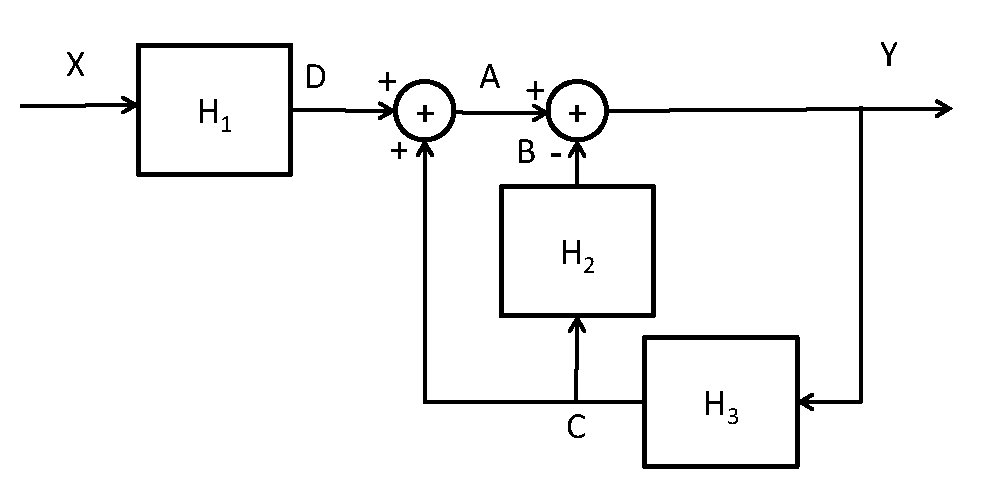
\includegraphics[width=.8\textwidth]{fig2.eps}
\end{figure}

For simplicity we have omitted all the terms $(e^{j\omega})$ in the diagram above. Unless otherwise stated uppercase letters will denote Fourier-domain variables and lower-case letters time-domain ones. We can now write all the system equations in Fourier domain:

\begin{eqnarray}
Y &=& A-B\label{eq1}\\
A &=& D+C\label{eq2}\\
B &=& H_2\cdot C\label{eq3}\\
C&=&H_3\cdot Y\label{eq4}\\
D&=&H_1 \cdot X\label{eq5}
\end{eqnarray}

The overall frequency response is defined as $H=\frac{Y}{X}$. Therefore, we need to combine the five equations above into a single one that has only $X$ and $Y$ as unknowns. Combining Eqs.~\ref{eq1},~\ref{eq2} and~\ref{eq3} we obtain:

\begin{equation}\label{eq6}
Y = D + (1-H_2)C
\end{equation}

Now combining Eq.~\ref{eq6} with Eqs.~\ref{eq4} and~\ref{eq5} we get to:

\begin{equation}\label{eq7}
Y = H_1\cdot X + (1-H_2)H_3 Y
\end{equation}

which has only two unknowns: $X$ and $Y$. Reorganizing Eq.~\ref{eq7} we finally obtain the overall frequency response of the system:

\begin{equation}
Y = \frac{H_1}{1+H_3(H_2-1)}X \Rightarrow H(e^{j\omega})=\frac{Y(e^{j\omega})}{X(e^{j\omega})}=\frac{H_1(e^{j\omega})}{1+H_3(e^{j\omega})(H_2(e^{j\omega})-1)}
\end{equation}

\emph{Finding the expression above: 3 exam points.}

\emph{Hint for future exams: Do not attempt to solve this type of problems by finding directly a time-domain expression relating $y[n]$ and $x[n]$ and then transforming such expression to the Fourier domain. This path is much more complex and will most likely lead you to mistakes, specially when feedback loops are involved. }

\vspace{1cm}

\textbf{(b)}

In order to determine the overall frequency response we just need to find the frequency response of the three sub-systems involved: $h_1[n]$, $h_2[n]$ and $h_3[n]$. For this, recall that the Z-transform of the sequence $g[n]=(0.5)^n \mu[n]$ is:

\begin{equation}
g[n]=(0.5)^n \mu[n] \stackrel{Z}{\longrightarrow} G(z)=\frac{1}{1-0.5 z^{-1}} \qquad ROC\equiv |z|>0.5
\end{equation}

Since $h_1[n]=(0.5)^{n}\mu[n-3]=(0.5)^3(0.5)^{n-3}\mu[n-3]$, its Z-transform is:

\begin{equation}
H_1(z)=(0.5)^3z^{-3}G(Z)=(0.5)^3z^{-3}\frac{1}{1-0.5 z^{-1}} \qquad ROC\equiv |z|>0.5
\end{equation}

Now, because the ROC of $H_1(z)$ includes the unit circle, the Fourier transform of $h_1[n]$ exists and takes the value:

\begin{equation}
H_1(e^{j\omega})=H_1(z)|_{z=e^{j\omega}}=(0.5)^3e^{-j3\omega}\frac{1}{1-0.5 e^{-j\omega}}
\end{equation}


The Fourier transforms of $h_2[n]$ and $h_3[n]$ are trivial:

\begin{eqnarray}
H_2(e^{j\omega})&=&1+2e^{-j2\omega}\\
H_3(e^{j\omega})&=&-e^{-j\omega}
\end{eqnarray}

So we can finally write that the overall frequency response of the system is:

\begin{equation}\label{eq:freqresponse}
H(e^{j\omega})=(0.5)^3\frac{e^{-j3\omega}}{(1-2e^{-j3\omega})(1-0.5e^{-j\omega})}
\end{equation}

\emph{Finding the expression above: 1 exam point.}

Finding the impulse response of the system requires transforming Eq.~\ref{eq:freqresponse} to the time-domain. This was a relatively difficult question that was intended only for those students aiming at the highest grade. We start by transforming Eq.~\ref{eq:freqresponse} to the Z-domain:

\begin{equation}\label{eq:systemfunction}
H(z)=(0.5)^3\frac{z^{-3}}{(1-2z^{-3})(1-0.5z^{-1})}
\end{equation}

The denominator of $H(z)$ is a fourth order polynomial, which means that it will have four roots, i.e. our system function has four poles. Obvioulsy, one pole is located in $p_1=0.5$. The poles $p_2$, $p_3$ and $p_4$ are the roots of the polynomial $(1-2z^{-3})$. Finding the roots of third order polynomial can be tricky but in this case, we can easily find one of its roots (that is pole $p_2$):

\[
1-2z^{-3} = 0 \Rightarrow z^{-3}=\frac{1}{2}  \Rightarrow p_{2}=(2)^{\frac{1}{3}}=\sqrt[3]{2}
\]

and therefore, we can factorize the term $1-2z^{-3}$ as:

\[
(1-2z^{-3})=(1-\sqrt[3]{2}z^{-1})Q(z)
\]

where $Q(z)=\frac{(1-2z^{-3})}{(1-\sqrt[3]{2}z^{-1})}$ must be a second-order polynomial. In order to find $Q(z)$ we use long division:

\begin{tabular}{r|cllll}
&\qquad& $\sqrt[3]{4}z^{-2}$ & $+\sqrt[3]{2}z^{-1}$ & $+1$&\\
\cline{2-6}
\\
$-\sqrt[3]{2}z^{-1}+1$ && $-2z^{-3}$ & $+0z^{-2}$&$+0z^{-1}$&$+1$\\
&& $-2z^{-3}$ & $+\sqrt[3]{4}z^{-2}$&&\\
\cline{3-6}\\
&&&$-\sqrt[3]{4}z^{-2}$&$+0z^{-1}$&$+1$\\
&&&$-\sqrt[3]{4}z^{-2}$&$+\sqrt[3]{2}z^{-1}$&\\
\cline{4-6}\\
&&&&$-\sqrt[3]{2}z^{-1}$&$+1$\\
&&&&$-\sqrt[3]{2}z^{-1}$&$+1$\\
\cline{5-6}\\
&&&&&$0$\\
\end{tabular}

As expected, the remainder of the division is zero and $Q(z)=\sqrt[3]{4}z^{-2}+\sqrt[3]{2}z^{-1}+1$ is a second degree polynomial. Now, we can easily find the two roots of $Q(z)$, which will correspond to the two remaining poles $p_3$ and $p_4$. By making the variable change $x=z^{-1}$ we find that:

\[
\sqrt[3]{4}x^{2}+\sqrt[3]{2}x+1=0 \Rightarrow x = \frac{-\sqrt[3]{2}\pm j\sqrt{3}\sqrt[6]{4}}{2\sqrt[3]{4}}
\]

and then by reversing the variable change ($z=x^{-1}$) we obtain that the two poles that we were looking for are:

\[
\begin{array}{lllll}
p_3&=& \frac{2\sqrt[3]{4}}{-\sqrt[3]{2}+ j\sqrt{3}\sqrt[6]{4}}=-0.63-1.09j\\
p_4&=& \frac{2\sqrt[3]{4}}{-\sqrt[3]{2}- j\sqrt{3}\sqrt[6]{4}}=-0.63+1.09j\\
\end{array}
\]

Always, when a fractional Z-transform has complex poles they will be in conjugate pairs, i.e. $p_4=p_3^*$ in this case. So we can write the system function in Eq.~\ref{eq:systemfunction} as:

\[
H(z)=(0.5)^3\frac{z^{-3}}{(1-p_1z^{-1})(1-p_2z^{-1})(1-p_3z^{-1})(1-p_3^*z^{-1})} \qquad ROC \equiv |z|>\sqrt[3]{2}
\]

Because all the elements of the overall system are causal, the overall system is also causal and, therefore, the ROC of $H(z)$ must be the region outside the circunference in which the largest (in absolute value) pole is located. Now, using fractional expansion:

\[
H(z) = (0.5)^3 \left[\frac{A}{1-p_1z^{-1}}+\frac{B}{1-p_2z^{-1}}+\frac{C}{1-p_3z^{-1}}+\frac{C^*}{1-p_3^*z^{-1}}+\right]
\]

where $p_1=0.5$, $p_2=\sqrt[3]{2}=1.26$ and $p_3=-0.63-1.09j$ and the residuals are:

\begin{equation}
\begin{array}{lllll}
A &=& \left.\left[(1-p_1z^{-1})H(z)\right]\right|_{z=p_1}&=&-0.53\\
B &=& \left.\left[(1-p_2z^{-1})H(z)\right]\right|_{z=p_2}&=&0.28\\
C &=& \left.\left[(1-p_3z^{-1})H(z)\right]\right|_{z=p_3}&=&0.13+0.04j\\
\end{array}
\end{equation}

Now we can finally invert $H(z)$ taking into account that all the poles correspond to causal components of the system:

\begin{equation}\label{impulse}
h[n] = (0.5)^3\cdot\left[A(p_1)^n+B(p_2)^n\mu[n]+C(p_3)^n\mu[n]+C^*(p_3^*)^n\mu[n]\right]
\end{equation}

\emph{Describing the steps needed to reach the expression above: 1 exam point. Computing the actual values of the residuals and the poles was not required.}

\emph{Hints for future exams: 
\begin{itemize}
\item Whenever the denominator of a irreducible fractional Z-transform is of degree greater than 2 and/or there are complex poles performing the inverse Z-transform becomes more tedious so if you find this type of problem in future exams leave it for the end, specially when there is only 1 exam point at stake.
\item You do not need to compute the actual values of the poles and/or the residuals. It is enough to CLEARLY describe the process and leave indicated the computations, as was mentioned in the solution to question 4 of the second toy exam available in the course web-page.
\item The expression in Eq.~\ref{impulse} can be re-written using only real terms. Although this was not required in the exam you can try to do it as an exercise. You can easily do it by expressing $p_3$, $p_3^*$, $C$, and $C^*$ in their polar form.
\end{itemize}
}


\vspace{1cm}

\textbf{QUESTION 2 (6 point):} A major problem in the recording of electrocardiograms (ECGs) is the appearance of unwanted 50-Hz interference in the output. The causes of this power line interference include magnetic induction, displacement currents in the leads on the body of the patients, and equipment interconnections. Assume that the bandwidth of the signal of interest is 1 KHz, that is $X_a(f)=0 \quad |f|>1000$ Hz. The analog signal is converted into a discrete-time signal with an ideal A/D converter operating using a sampling frequency $f_s$. The resulting signal $x(n)=x_a(nTs)$ is then processed with a discrete-time system that is described by the difference equation:

\[
y[n] = x[n]+ax[n-1]+bx[n-2]
\]

The filtered signal, $y(n)$, is then converted back into an analog signal using an ideal D/A converter. Design a system for removing the 50-Hz interference by specifying values for $fs$, $a$, and $b$ so that a 50-Hz signal of the form  will not appear in the output of the D/A converter. (Hint: The interference will be removed if the filter has a transfer function equal to zero for the corresponding radian frequency). 


\vspace{1cm}


\textbf{SOLUTION:}

To avoid aliasing the sampling period has to satisfy the Nyquist criterion: $T_s\leq 5\cdot 10^{-4}$ seconds. 

\emph{Giving a valid sampling rate: 2 points}.

From the solution of problem 2 of classroom exercise 3 (available in the course web-page) we can see that the inteference will be removed if:

\begin{eqnarray}
a &=& -2\cos (\omega_\epsilon)\\
b &=& 1
\end{eqnarray}

where $\omega_\epsilon$ is the discrete-time frequency of the interference. That is, assuming that we sampled at the Nyquist rate:

\[
\omega_\epsilon=50\cdot 2\pi \cdot T_s=0.05\pi
\]

\emph{Expression of a and b: 4 points}.

\emph{Hint for future exams: This problem is identical to problem 2 of exercise 3 (see the course web-page). Very few students attending this exam managed to solve this problem even though in the hints for the exam that were given in the course web-page it was specifically said that you should check the solutions to the problems of exercise 3. Next time you should really pay attention to the hints!.} 


\vspace{1cm}

\textbf{QUESTION 3 (5 points):} Consider the system shown in the figure below:

\begin{figure}[h!]
\centering
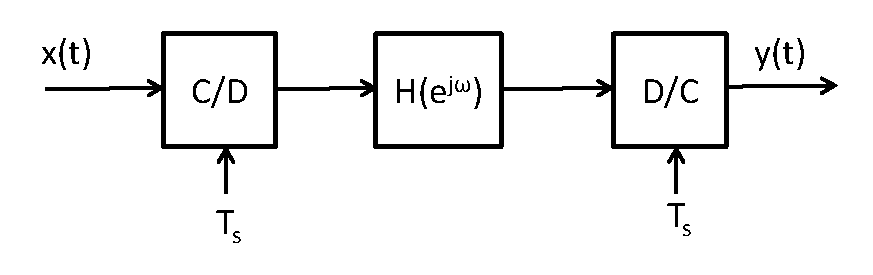
\includegraphics[width=.8\textwidth]{fig3.eps}
\end{figure}

\begin{itemize}
\item[(a)] (2 points) If $x(t)$ is bandlimited to $10$ KHz, what is the maximum value of the sampling period that can be used to avoid aliasing?
\item[(b)] (3 points) Given the Fourier transform of $x[n]$ is as shown on the left figure below, it is desired to obtain $y[n]$ with Fourier transform as shown on the right figure below. Specify the impulse response $h[n]$ of the discrete-time system $H(e^{j\omega})$. Hint: Use the frequency shift property of the Fourier transform.
\end{itemize}

\begin{figure}[h!]
\centering
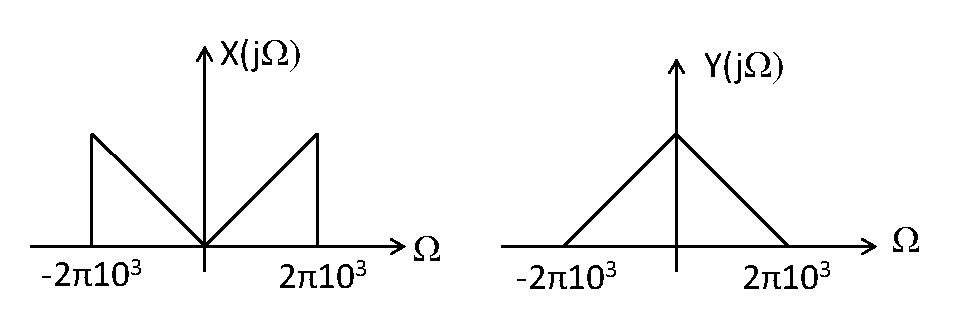
\includegraphics[width=.8\textwidth]{fig4.eps}
\end{figure}

\vspace{1cm}

\textbf{SOLUTION:}

\textbf{(a)}

Obviously the maximum value of the sampling period is determined by the Nyquist criterion $T_s<\frac{1}{2f_{max}}=\frac{1}{2\cdot 10^4}=5\cdot 10^{-5}$ seconds.

\emph{Giving the minimum sampling period: 2 points}


\textbf{(b)}

Because it is not specifically said in part (b) that the sampling period of the system has to be equal to that of part (a) we can just set the sampling frequency of our system to $T_s=5\cdot 10^{-4}$. Then, the DTFT of the discrete-time sequence $x[n]$ looks like is shown in the figure below:

\begin{figure}[h!]
\centering
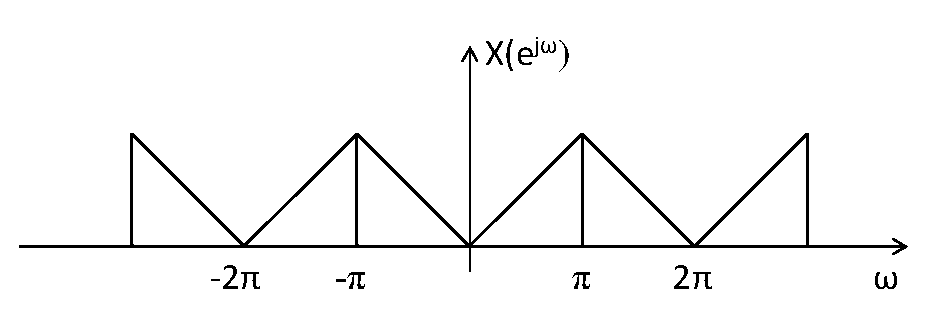
\includegraphics[width=.8\textwidth]{ex3sol1fig1.eps}
\end{figure}

Clearly, in order to obtain the desired output spectrum we need to shift the DTFT above by $\pi$ radians/second. In order to produce a frequency shift of $\omega_0$ radians/second in a given real sequence $x[n]$ the only possibility is to multiply it by a modulation sequence (one or more complex exponentials). In the simplest case such modulation sequence is the complex sequence $m_c[n]=e^{j\omega_0 n}$, as told by the shifting property of the Fourier transform. A better alternative would be to use the real modulation sequence $m_r[n]=\frac{1}{2}\left(e^{j\omega_0 n}+e^{-j\omega_0 n}\right)=cos(\omega_0 n)$. Because the input sequence $x[n]$ is real its DTFT satifies the symmetry property $X(e^{j\omega})=X^*(e^{-j\omega})$. Thus, multiplying the real sequence $x[n]$ by either $m_c[n]$ or $m_{r}[n]$ has the same effect of shifting the DTFT of $x[n]$ by $\omega_0$ radians/second. Anyway, consider the case that we used $m_{r}[n]$. Then the input-output relationship of the required discrete-time system is:

\begin{equation}\label{eq:inout}
y[n] = cos(\omega_0 n)\cdot x[n]=cos(\pi n)\cdot x[n]=(-1)^n x[n]
\end{equation}

So that the DTFT of $y[n]$ will look like this:

\begin{figure}[h!]
\centering
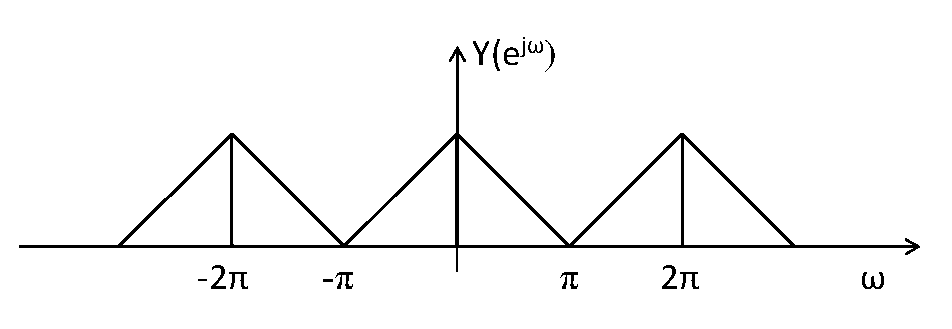
\includegraphics[width=.8\textwidth]{ex3sol1fig2.eps}
\end{figure}

And then, after the D/C converter, the Fourier transform of the analog signal $y(t)$ will just look just like the one given in the problem description. 

\emph{Reaching this point was enough for getting the 3 points. Actually we were very flexible in the correction of this problem and just stating the frequency shifting property of the DTFT was enough for getting 1 point.} 

The perfect solution goes just a bit further. The problem was asking us for the impulse response of the discrete-time system described by the input-output relationship in Eq.~\ref{eq:inout}. It is obvious that such system \textbf{is not time-invariant}. Therefore, the perfect answer was to say that because the required system is time-variant its corresponding impulse response is also time-variant. That is for the time-instant $k$ the impulse response of the system is: $h_k[n]=(-1)^k \delta[n]$. So for even time-instants the impulse response is $h_{even}[n]=\delta[n]$ and for odd time-instants the impulse response is $h_{odd}[n]=-\delta[n]$.

NOTE: If you would have used the same sampling period as in part (a), that is $T_s=5\cdot 10^{-5}$ then there would be a gap between the spectral aliases in $X(e^{j\omega})$. Thus the optimal discrete time system would have consisted of a downsampler by a factor 10, the system described by Eq.~\ref{eq:inout} and an upsampler by a factor 10. This was a bit longer path but also completely valid.


%It is clear that our system has to produce a frequency shift in the input signal. In order to produce a frequency shift of $\omega_0$ radians/second in a given real sequence $x[n]$ the only possibility is to multiply it by a modulation sequence. In the simplest case such modulation sequence is the complex sequence $m_c[n]=e^{j\omega_0 n}$. Of course, a better alternative would be to use the real modulation sequence $m_r[n]=\frac{1}{2}\left(e^{j\omega_0 n}+e^{-j\omega_0 n}\right)=cos(\omega_0 n)$. Because of the input sequence $x[n]$ is real its DTFT satifies the symmetry property $X(e^{j\omega})=X^*(e^{-j\omega})$. Thus, multiplying the real sequence $x[n]$ by either $m_1[n]$ or $m_{2}[n]$ has the same effect of shifting the DTFT of $x[n]$ by $\omega_0$ radians/second. Anyway, consider the case that we used $m_{2}(e^{j\omega})$
%
%\[
%y[n] = e^{j\omega n}x[n]
%\]
%
%Cleary, such a system is not time-invariant and therefore the impulse response depends on the actual value of the time instant (index $n$). This solution is not rigourously right because it was not said in the problem description that the resulting system had to be time-invariant and therefore the impulse response could vary with respect to the time-index. However, it is a valid argumentation and this solution was awarded \emph{3 points}.
%
%
%
%The hint tells that we should try to use the frequency shifting property of the Fourier transform, that is, in the discrete Fourier transform domain:
%
%\begin{equation}\label{eq:freqshift}
%y[n] = e^{j\omega_0 n}x[n] \Rightarrow Y(e^{j\omega})=X(e^{j(\omega-\omega_0)})
%\end{equation}
%
%If we consider that the Nyquist rate is used in the system ($T_s=5\cdot 10^{-5}$ seconds) then the DTFT of $x[n]$ looks like shown below:
%
%
%\begin{figure}[h!]
%\centering
%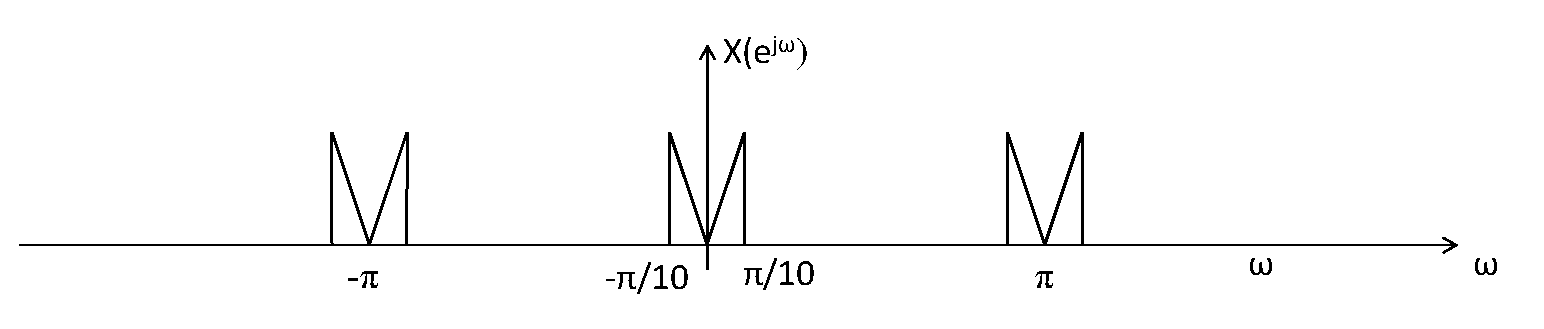
\includegraphics[width=\textwidth]{fig5.eps}
%\end{figure}
%
%Clearly, before trying to express $Y(e^{j\omega})$ as a frequency shifted version of $X(e^{j\omega})$ we need to expand $X(e^{j\omega})$ by a factor of 10 so that there will not be any gab between the spectral aliases. This can be achieved by using a decimator (with $L$=10) after the C/D block. The spectrum of the output $v[n]$ of such decimator will look like:
%
%
%\begin{figure}[h!]
%\centering
%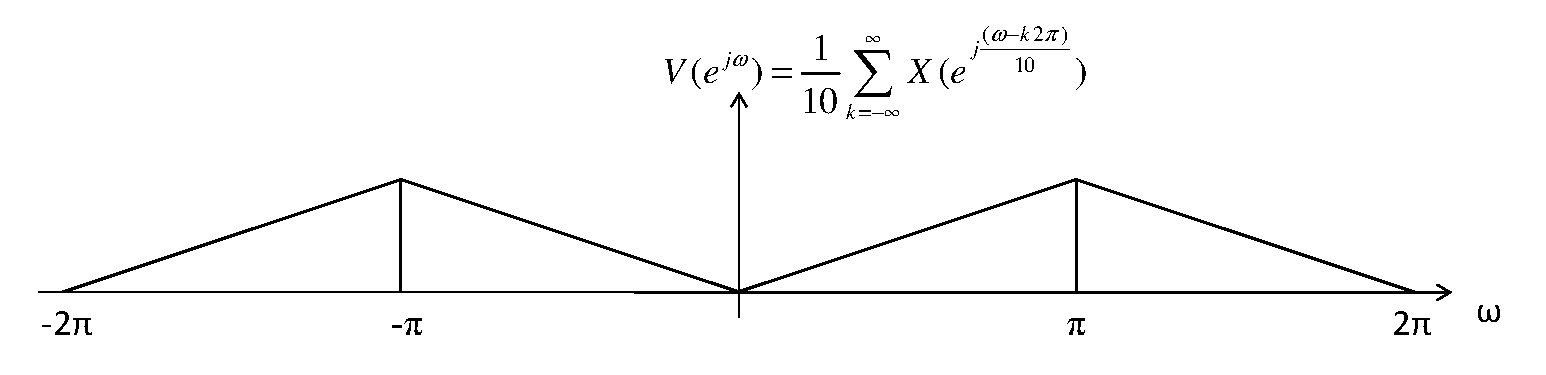
\includegraphics[width=\textwidth]{fig6.eps}
%\end{figure}
%
%Now to get closer to the desired output we need to shift the spectrum of $v[n]$ by a factor equal to $\pi$. Indeed, this can be obtained by multiplying $v[n]$ with the complex signal $m[n]=10\cdot e^{j\pi n}$ (this is a valid solution). The factor 10 is to compensate the multiplying factor $\frac{1}{10}$ introduced by the decimator. A better solution is to use the real sequence $m[n]=5\left(e^{j\pi n}+e^{-j\pi n}\right)=10 \cos (\pi n)=10\cdot(-1)^n$. Using the frequency shift property in Eq.~\ref{eq:freqshift}, one can easily check that the spectrum of $w[n]=v[n]\cdot m[n]$ is as depicted below:
%
%
%\begin{figure}[h!]
%\centering
%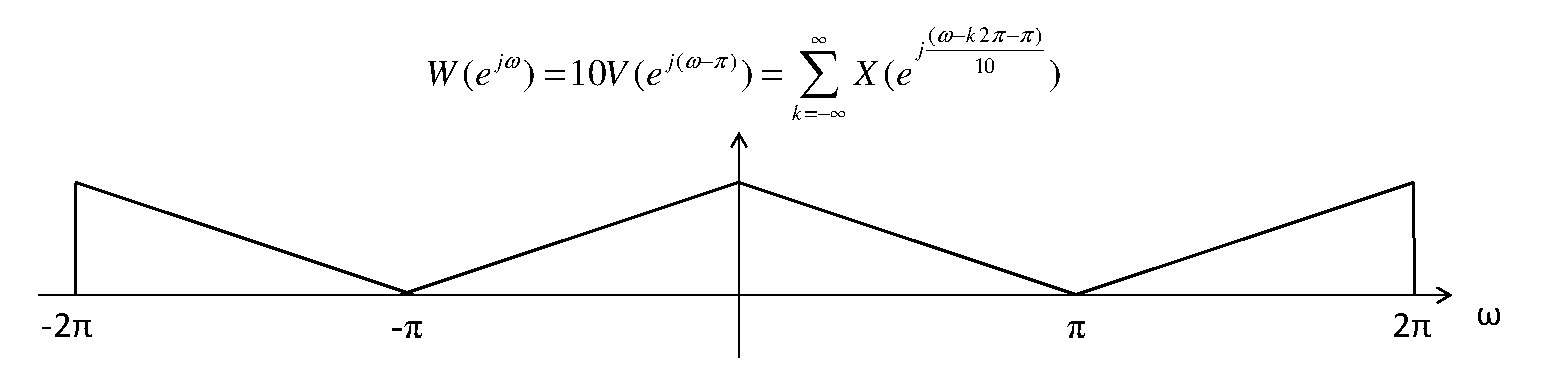
\includegraphics[width=\textwidth]{fig7.eps}
%\end{figure}
%
%And finally, the only thing that we need to do is to compress the spectrum of $\W(e^{j\omega})$ by a factor of 10. This can be achieved by using an upsampler (with $M=10$). The spectrum of the output sequence ($r[n]$) of the upsampler will be as shown in the figure below:
%
%\begin{figure}[h!]
%\centering
%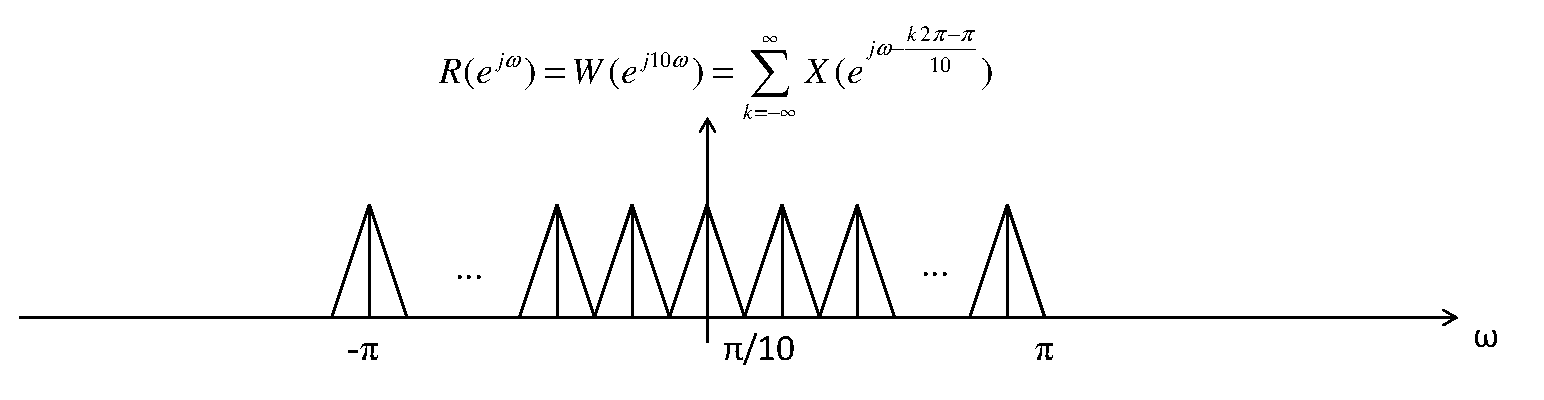
\includegraphics[width=\textwidth]{fig8.eps}
%\end{figure}
%
%The reconstruction filter will only keep the baseband spectral alias in the figure above and, therefore, the CTFT of the output analog signal will be as required in the problem description.



\vspace{1cm}

\textbf{QUESTION 4 (5 points):} Calculate the convolution of the following three sequences using the Z-transform:

\begin{eqnarray}
x_1[n]&=&2^n\mu[n]\\
x_2[n]&=&\delta[n]+2\delta[n-1]\\
x_3[n]&=&\delta[n]-3\delta[n+1]
\end{eqnarray}


\vspace{1cm}

\textbf{SOLUTION:}

Because the problem asks to use the Z-transform this means that we have to find the convolution using the following relationship:

\begin{equation}
y[n]=x_1[n]\otimes x_2[n] \otimes x_3[n] = Z^{-1}\left\{X_1(z)X_2(z)X_3(z)\right\}\\
\end{equation}

First we compute the Z-transform of the three given sequences. This is a trivial task using the table of Z-transform pairs in the summary of chapter 6:

\begin{equation}
\begin{array}{llll}
X_1(z)&=&\frac{1}{1-2z^{-1}} & \textrm{ROC} \equiv |z|>2\\
X_2(z)&=&1+2z^{-1} & \textrm{ROC} \equiv z\neq 0\\
X_3(z)&=&1-3z & \textrm{ROC} \equiv z\neq \infty
\end{array}
\end{equation}

So we need to invert the following Z-transform:

\begin{equation}\label{eq:Yz}
Y(z)=\frac{(1+2z^{-1})(1-3z)}{1-2z^{-1}}=\frac{-5-3z+2z^{-1}}{(1-2z^{-1})} \qquad \textrm{ROC}\equiv |z|>2 
\end{equation}

\emph{Reaching Eq.~\ref{eq:Yz} was already granted 2 points.}

Notice that this Z-transform is already directly invertible using the shifting property of the Z-transform (without needing to compute residuals or long division):

\[
Y(z)=-5\underbrace{\frac{1}{1-2z^{-1}}}_{G(z)}-3z\underbrace{\frac{1}{1-2z^{-1}}}_{G(z)}+2z^{-1}\underbrace{\frac{1}{1-2z^{-1}}}_{G(z)}
\]

So we finally obtain that:

\begin{equation}\label{eq:yn}
y[n] = -5(2)^n\mu[n]-3(2)^{n+1}\mu[n+1]+2(2)^{n-1}\mu[n-1]
\end{equation}

\emph{Reaching Eq.~\ref{eq:yn} was granted 3 points.}




\vspace{1cm}

\textbf{QUESTION 5 (3 points):} Find the region of convergence of the Z-transform of the following sequences:

\begin{itemize}
\item[(a)] (1 point) $x_a[n]=\left(\frac{1}{4}\right)^n\mu[n]+\left(\frac{1}{2}\right)^{2n}\mu[-n]$
\item[(b)] (1 point) $x_b[n]=\left\{\begin{array}{lll}1 &\quad& -15 \leq n \leq -5\\0 &\quad& \textrm{otherwise} \end{array}\right.$
\item[(c)] (1 point) $x_c[n]=2^n\mu[-n-5]$
\end{itemize}

\vspace{1cm}

\textbf{SOLUTION:}

\textbf{(a)}

\[
x_{a}[n]=\left(\frac{1}{4}\right)^n\mu[n]+\left(\frac{1}{2}\right)^{2n}\mu[-n]=\underbrace{\left(\frac{1}{4}\right)^n\mu[n]}_{\textrm{ROC}\equiv |z|<\frac{1}{4}}+\underbrace{\left(\frac{1}{4}\right)^{n}\mu[-n]}_{\textrm{ROC}\equiv |z|>\frac{1}{4}}
\]

Obviously, the ROC of the causal and anti-causal components of $x_a[n]$ do not overlap and therefore their intersection is empty. Thus $X_a(z)$ does not converge for any value of $z$, i.e. ROC $\equiv \emptyset$

\textbf{(b)}

Because the sequence $x_b[n]$ is of finite duration its ROC must be all z-plane except possibly $z=0$ or $z=\infty$. Because the sequence is anti-causal its Z-transform will contain only positive powers of $z$ which means that it will converge for $z=0$ but not for $z=\infty$. Thus the ROC of this sequence is the whole z-plane except $z=\infty$.

\textbf{(c)}

Using the formula of the Z-transform:

\[
X_c(z)=\sum_{n=-\infty}^{\infty}x_c[n]z^{-n}=\sum_{n=-\infty}^{-5}2^nz^{-n}=\sum_{n=5}^{\infty}2^{-n}z^n=\sum_{n=5}^{\infty}(2^{-1}z)^n
\]

The summatory above will converge only if $|2^{-1}z|<1$ which means that the ROC must be $|z|<2$.

You could have reached the same result using this alternative way:

\[
x_c[n]=2^n\mu[-n-5]=2^n\mu[-(n+1+4)]=2^{-4}\underbrace{2^{n+4}\mu[-(n+1+4)]}_{-g[n+4]}
\]

So the z-transform of $x_c[n]$ will be:

\[
X_c(z)=-2^{-4}z^{4}G(z)
\]

which means that $X_c(z)$ will not converge for $z=\infty$ nor for any value of $z$ for which $G(z)$ does not converge. Using the Z-transform pairs table we know that the ROC of $g[n]=-2^n\mu[n-1]$ is $|z|<2$. Therefore, the ROC of $X_c(z)$ must be $|z|<2 \cap z\neq \infty \Rightarrow \textrm{ROC} \equiv |z|<2$.

\vspace{1cm}

\textbf{QUESTION 6:} A signal $x[n]$ has been passed through a causal LTI system given by the following difference equation:

\[
y[n]-y[n-1]+\frac{1}{4}y[n-2]=2x[n]-2x[n-1]-\frac{11}{4}x[n-2]+3x[n-3]-\frac{3}{4}x[n-4]
\]

Find the impulse response of the system (4 points). Is the system stable (1 point)? Could $x[n]$ by recovered from $y[n]$ using a realizable filter (1 point)?

\vspace{1cm}

\textbf{SOLUTION:}

Using the shifting property of the Z-transform we easily obtain that:

\begin{equation}\label{hz}
H(z)=\frac{Y(z)}{X(z)}=\frac{2-2z^{-1}-\frac{11}{4}z^{-2}+3z^{-3}-\frac{3}{4}z^{-4}}{1-z^{-1}+\frac{1}{4}z^{-2}}
\end{equation}

Clearly, we cannot invert $H(z)$ directly because the numerator does not look anything like $(1-\alpha z^{-1})$ or $(1-\alpha z^{-1})^2$. Therefore a valid approach would be to use long division and subsequently the method of the residuals to express $H(z)$ as a linear combination of powers of $z$ and terms having as denominator either $(1-\alpha z^{-1})$ or $(1-\alpha z^{-1})^2$. We will explore this approach later. 

However, because the denominator of our fractional Z-transform is of order 2 it is worth checking if its two roots are identical (i.e. if we have a double pole), which would make the denominator of $H(z)$ become $(1-\alpha z^{-1})^2$ with $\alpha$ equal to the value of the double pole. Then $H(z)$ would be directly invertible using the shifting property of the Z-transform. To explore this possibility, we start by finding the poles of $H(z)$, that is, the roots of the polynomial $1-z^{-1}+\frac{1}{4}z^{-2}$. To do this we make the variable change $x=z^{-1}$ and solve:

\[
1-x+\frac{1}{4}x^{2}=0
\]

obtaining the solutions $x_1=x_2=2$. Reversing the variable change we obtain the roots of our polynomial in $z^{-1}$ are $z_1=z_2=\frac{1}{x1}=\frac{1}{2}$. So we have obtained that $H(z)$ effectively has a double pole at $z=\frac{1}{2}$ and therefore we can write $H(z)$ as:

\begin{equation}\label{eq:hz}
H(z)=\frac{Y(z)}{X(z)}=\frac{2-2z^{-1}-\frac{11}{4}z^{-2}+3z^{-3}-\frac{3}{4}z^{-4}}{(1-\frac{1}{2}z^{-1})^2} \qquad \textrm{ROC}\equiv |z|>\frac{1}{2}
\end{equation}

Notice that we know that the ROC of $H(z)$ is $|z|>\frac{1}{2}$ because it is said in the problem description that the system is causal. From here we can already use the table of Z-transform pairs and the shifting property of the Z-transform to obtain an expression of $h[n]$. Recall from the table of Z-transform pairs:

\begin{equation}
g[n] = n\left(\frac{1}{2}\right)^n\mu[n] \Rightarrow G(z)=\frac{\frac{1}{2}z^{-1}}{(1-\frac{1}{2}z^{-1})^2}
\end{equation}

Clearly we can write the expression of $H(z)$ in Eq.~\ref{eq:hz} as:


\[
H(z)=4zG(z)-4G(z)-\frac{11}{2}z^{-1}G(z)+6z^{-2}G(z)-\frac{3}{2}z^{-3}G(z)
\]

And therefore:

\begin{equation}\label{eq:hn1}
\begin{array}{lll}
h[n]&=&4(n+1)\frac{1}{2}^{(n+1)}\mu[n+1]-4n\left(\frac{1}{2}\right)^n\mu[n]-\frac{11}{2}(n-1)\left(\frac{1}{2}\right)^{(n-1)}\mu[n-1]\\
&&+6(n-2)\left(\frac{1}{2}\right)^{(n-2)}\mu[n-2]-\frac{3}{2}(n-3)\left(\frac{1}{2}\right)^{(n-3)}\mu[n-3]
\end{array}
\end{equation}

\emph{Reaching Eq.~\ref{eq:hn1} or an equivalent one was granted 4 points}.

Although this was not required in the exam, one can operate a bit more in order to express Eq.~\ref{eq:hn1} in this more compact form:

\begin{equation}\label{final}
h[n]=2\delta[n]-6\delta[n-2]+(1-n)\left(\frac{1}{2}\right)^n\mu[n-3]
\end{equation}

There was an alternative way of reaching the final solution. Because the numerator of $H(z)$ in Eq.~\ref{hz} is not of lower degree than the denominator we could have used long-division to express $H(z)$ as:

\begin{equation}\label{eq:zeros}
H(z)=1-3z^{-2} + \frac{1-z^{-1}}{\left(1-\frac{1}{2}z^{-1}\right)^2}
\end{equation}

Then we can express $H(z)$ as:

\[
H(z)=1-3z^{-2} + 2zG(z)-2G(z)
\]

with $G(z)=\frac{\frac{1}{2}z^{-1}}{(1-\frac{1}{2}z^{-1})^2}$. Thus the inverse Z-transform will be:

\begin{equation}
h[n]=\delta[n]-3\delta[n-2]+2\left(\frac{1}{2}\right)^{(n+1)}\mu[n+1]-2\left(\frac{1}{2}\right)^{n}\mu[n]
\end{equation}

which, operating a bit can be rewriten exactly as in Eq.~\ref{final}.

Is the system stable?

There are two alternative ways of anwering this question:
\begin{itemize}
\item Yes because the ROC of $H(z)$ ($|z|>\frac{1}{2}$) includes the unit circle.
\item Yes because the system is causal and all the poles of the system function are inside the unit circle.
\end{itemize}

\emph{Justifying properly your answer: 1 point}

Could $x[n]$ be recovered from $y[n]$ using a realizable filter?

We could recover $x[n]$ from $y[n]$ by passing $y[n]$ through a filter having as system function $H^{-1}(z)=\frac{1}{H(z)}$. Therefore, what they are asking here is whether the system $H^{-1}(z)$ is realizable, that is whether it is causal and stable. 

The zeros of $H(z)$ become poles in $\frac{1}{H(z)}$. From Eq.~\ref{eq:zeros} we can see that $H(z)$ has a double zero at $z=0$ and a zero at $z=1$. Therefore, $H^{-1}(z)$ has a double pole at $z=0$ and a pole at $z=1$. Because the pole at $z=1$ is not stricly inside the unit circle, the system $H^{-1}(z)$ will be unstable. Thus, $x[n]$ cannot be recovered from $y[n]$ using a realizable filter.

\emph{Justifying properly your answer: 1 point}

\end{document}